\section{Проектирование программного средства} % (fold)
\label{sec:arch_and_mod}

\subsection{Разработка программного развертывания}
\label{sub:arch_and_mod:graphlib}

Прежде чем приступать к непосредственной реализации программного средства, необходимо определиться с архитектурой коллективной работы с приложением.
Во-первых, необходимо провести анализ необходимой аппаратной конфигурации, на которой будут работать части конечного программного средства, и описать их взаимодействие между собой. Для описания узлов и их связей будем использовать диаграмму развертывания:
\begin{figure}[ht]
\centering
  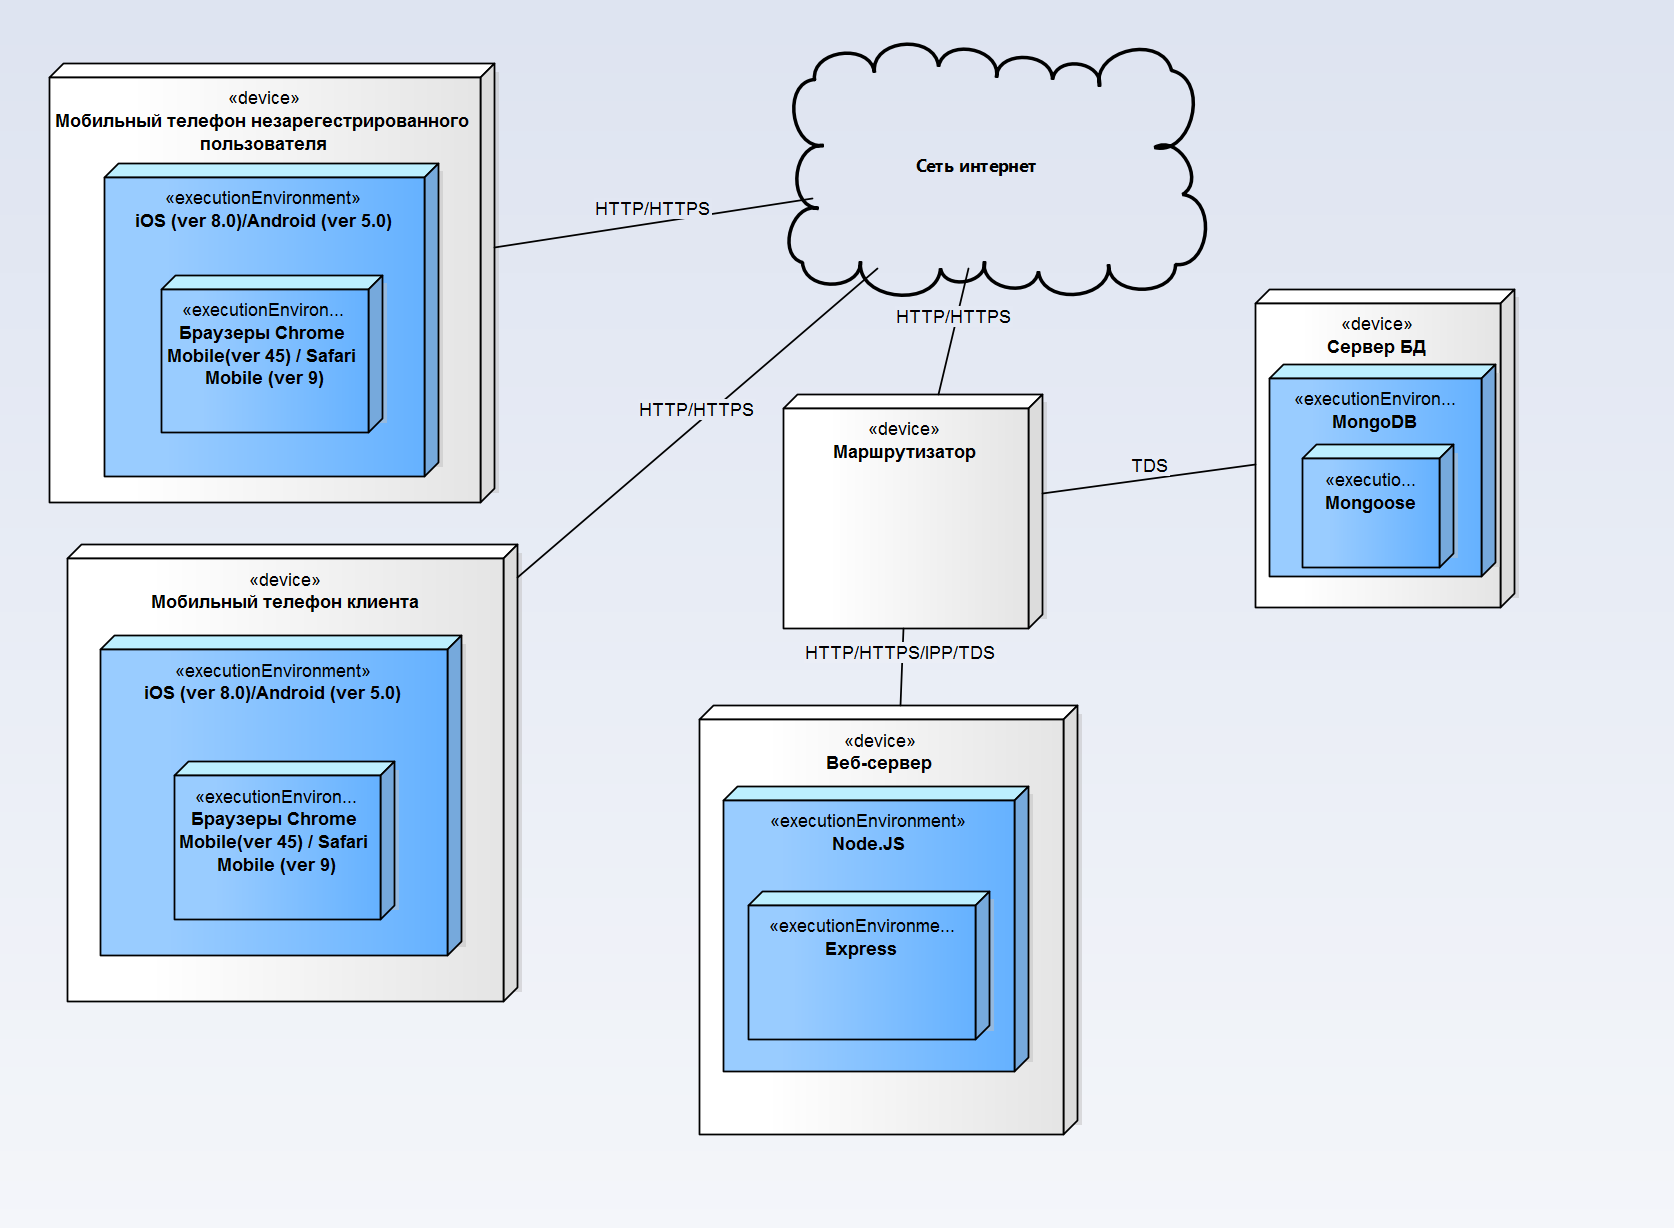
\includegraphics[scale=0.5]{device.png}  
  \caption{ Диаграмма развертывания. }
  \label{fig:domain:manual_structure:credit_device}
\end{figure}
На основе вышеизображенной диаграммы можно сделать следующие выводы:

\begin{enumerate}
  \item узлы могут располагаться в различных частях мира и взаимодействовать между собой через сеть Интернет;
  \item сервер базы данных поддерживаются в рабочем состоянии отдельно от основного сервера;
  \item клиент, осуществляющий работу с системой с помощью HTTP/HTTPS;
  \item HTTPS протокол применяется как к клиентам, так и к всевозможным серверам, для осуществления обмена запросами и ответами на них;
\end{enumerate}

\subsection{Разработка архитектуры БД }
\label{sub:arch_and_mod:graphlib}

Перед тем, как приступать к процессу разработки, сначала нужно смоделировать базу данных, которая является оcновой будущего приложения. Чтобы база данных не вызывала трудностей при работе с ней, когда будет заполнена информацией, крайне желательно, чтобы она соответствовала трем нормальным формам:
\begin{itemize}
  \item защита от CSRF-атак (cross-site request forgery, межсайтовая подделка запроса), при которых данные пользователя могут быть переданы на другой сайт (например, сайт злоумышленника или сайт платежной системы) для совершения некой вредоносной операции;
  \item Первая нормальная форма. Переменная отношения находится в первой нормальной форме тогда и только тогда, когда в любом допустимом значении отношения каждый его кортеж содержит только одно значение для каждого из атрибутов. 
  \item Вторая нормальная форма. Переменная отношения находится во второй нормальной форме тогда и только тогда, когда она находится в первой нормальной форме, и каждый неключевой атрибут функционально полно зависит от ее потенциального ключа.
  \item Третья нормальная форма. Переменная отношения находится в третьей нормальной форме тогда и только тогда, когда она находится во второй нормальной форме, и отсутствуют транзитивные функциональные зависимости неключевых атрибутов от ключевых.
\end{itemize}
В дипломном проекте будет разрабатываться нереляционная база данных. Делаться это будет путем создания JavaScript объектов, которые в последствии дополняться необходимыми полями и впоследствии будут хранится в базе данных также в виде объектов. Преимущества данного подхода являются: 
\begin{enumerate}
  \item решение проблемы масштабируемости;
  \item решение проблемы доступности;
  \item применение различных типов хранилищ;
  \item возможность создания базы данных без задания схемы;
  \item возможность использования многопроцессорности;
  \item сокращение времени разработки;
  \item скорость и производительность;
\end{enumerate}
Схема базы данных разрабатываемого приложения имеет следующий вид:
\begin{figure}[ht]
\centering
  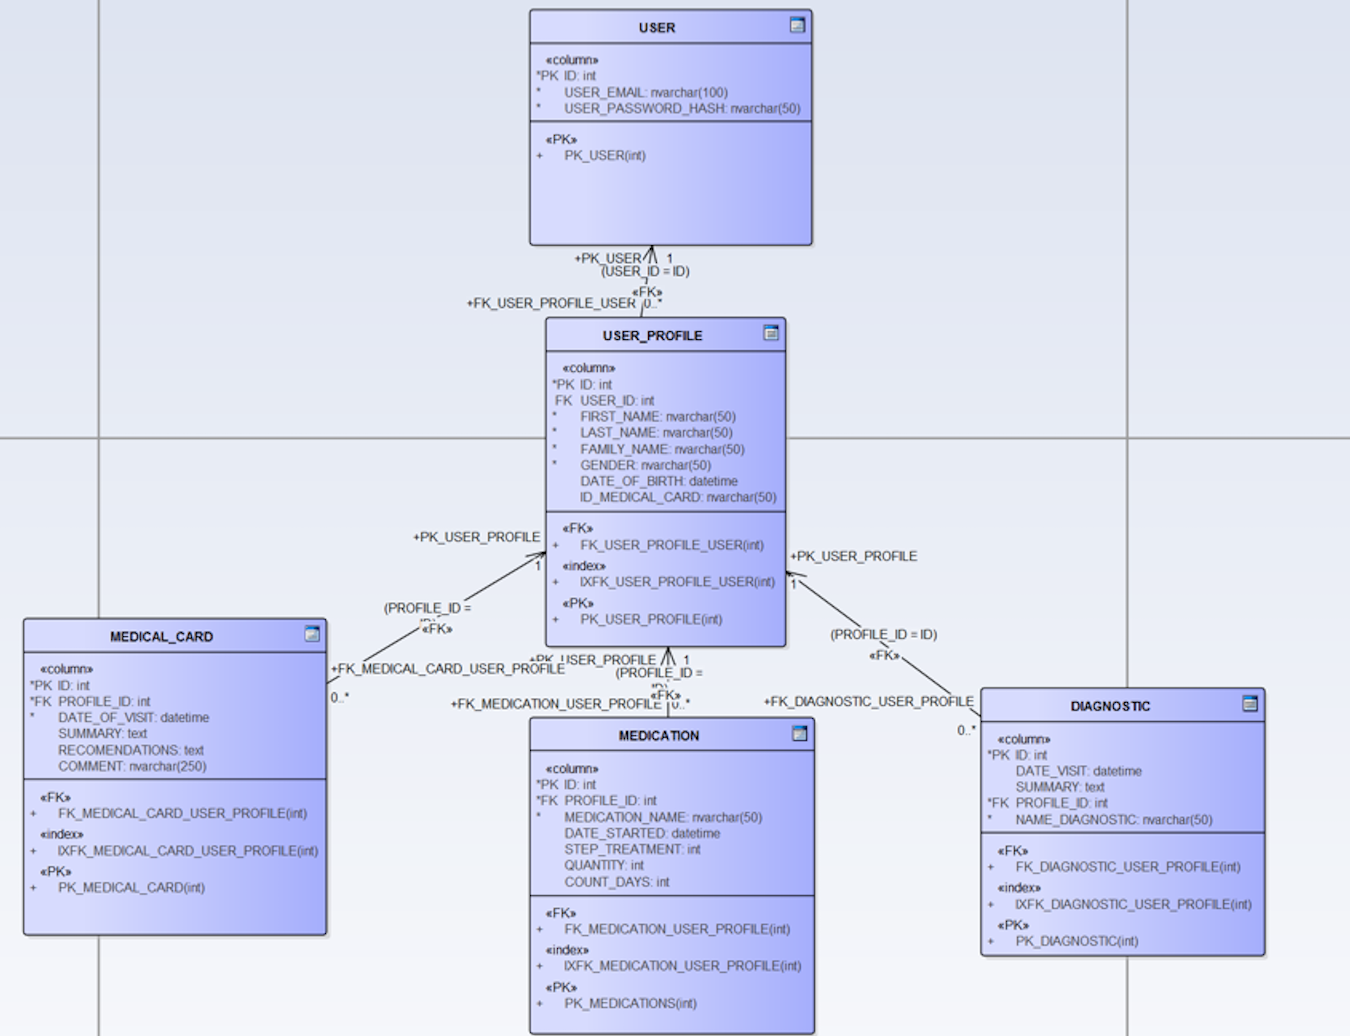
\includegraphics[scale=0.7]{db.png}  
  \caption{ Модель базы данных программного средства. }
  \label{fig:domain:manual_structure:credit_db}
\end{figure}

\subsection{Разработка алгоритма ПС }
\label{sub:arch_and_mod:alholib}
На рисунке ~\ref{fig:domain:manual_structure:alho_sp} представлена схема работы клиентского приложения, которая демонстрирует алгоритм работы программного средства в целом. Из схемы можно увидеть, что пользователь может взаимодействовать с двумя частями клиентского приложения:



\begin{enumerate}
  \item с модулем карточек, который позволяет взаимодействовать различными способами с карточками;
  \item с модулем работы с изображением;
\end{enumerate}
Веб-сервер приложения будет представлять собой приложение, построенное на концепции модифицированной архитектуры MVC со слоями:
\begin{enumerate}
  \item слой отражения модели на таблицу в базе данных(ML);
  \item слой доступа к данным (DAL)
  \item слой бизнес логики (BLL)
  \item слой управления (Controller)
\end{enumerate}
\begin{figure}[ht]
\centering
  \includegraphics[scale=0.4]{structurServer.png}  
  \caption{ Структура серверного-приложения при использовании модифицированной архитектуры MVC. }
  \label{fig:domain:manual_structure:structural_server}
\end{figure}

Слой управления представляет собой управленческий механизм, который обеспечивает связь между пользователем сервера и непосредственно самого сервера. Его основная задача отвечать на запросы пользователя и выдавать ему корректные результаты. Также одной из дополнительных функций - является контроль переданных данных от пользователя.

Слой доступа к данным предоставляет интерфейс для определенного рода операций взаимодействия внешних слоев с источником данных, в данном случае с объектами моделей.

Слой бизнес-логики описывает основные функции приложения, предназначенные для достижения поставленных перед ним целей.

Слой отраэения модели на таблицу в базе данных представляет собой совокупность объектов, связанных между собой и дополненных в последующем определенного вида параметрами для легкой доступности самих моделей.

На рисунке ~\ref{fig:domain:manual_structure:structural_server} представлена структура серверного-приложения на основе модифицированной MVC архитектуры. Такая структура имеет следующие преимущества:
\begin{itemize}
  \item подход позволяет производить параллельную разработку;
  \item возможность заменять слои, не нарушая тем самым целостность приложения;
  \item возможность протестировать каждый из слоев независимо друг от друга;
\end{itemize}

Клиентское приложение будет представлять собой приложение, построенное на концепции архитектуры Redux с основными принципами:
\begin{enumerate}
  \item состояние всего приложения сохранено в дереве объектов внутри одного хранилища (Store);
  \item единственный способ изменить состояние - это применить действие (Action);
  \item для определения трансформации хранилища используются чистые функции редьюсеры (Reducer);
\end{enumerate}
\begin{figure}[ht]
\centering
  \includegraphics[scale=0.5]{reduxFlow.png}  
  \caption{ Структура клиентского-приложения при использовании архитектуры Redux. }
  \label{fig:domain:manual_structure:structural_client}
\end{figure}

Действия - это структура, которая передает данные из приложения в хранилище. Они являются единственными источниками информации для хранилища. Действия яаляются обычными JavaScript объектами.

Редьюсер - чистая функция, которая принимает предыдущее состояние и действие и возвращает следующее состояние.

Хранилище - объект, который соеденяет все части вместе. Хранилище берет на себя следующие задачи:
\begin{itemize}
  \item содержать состояние приложения (state);
  \item предоставлять доступ к состоянию приложения;
  \item предоставлять возможность обновления состояния;
\end{itemize}

На рисунке ~\ref{fig:domain:manual_structure:structural_client} представлена структура клиентского-приложения она имеет следующие преимущества:
\begin{itemize}
  \item позволяет использовать компонентный подход в разработке;
  \item делает изменение состояние предсказуемым;
  \item позволяет использовать функциональный подход;
\end{itemize}
\begin{figure}[ht]
\centering
  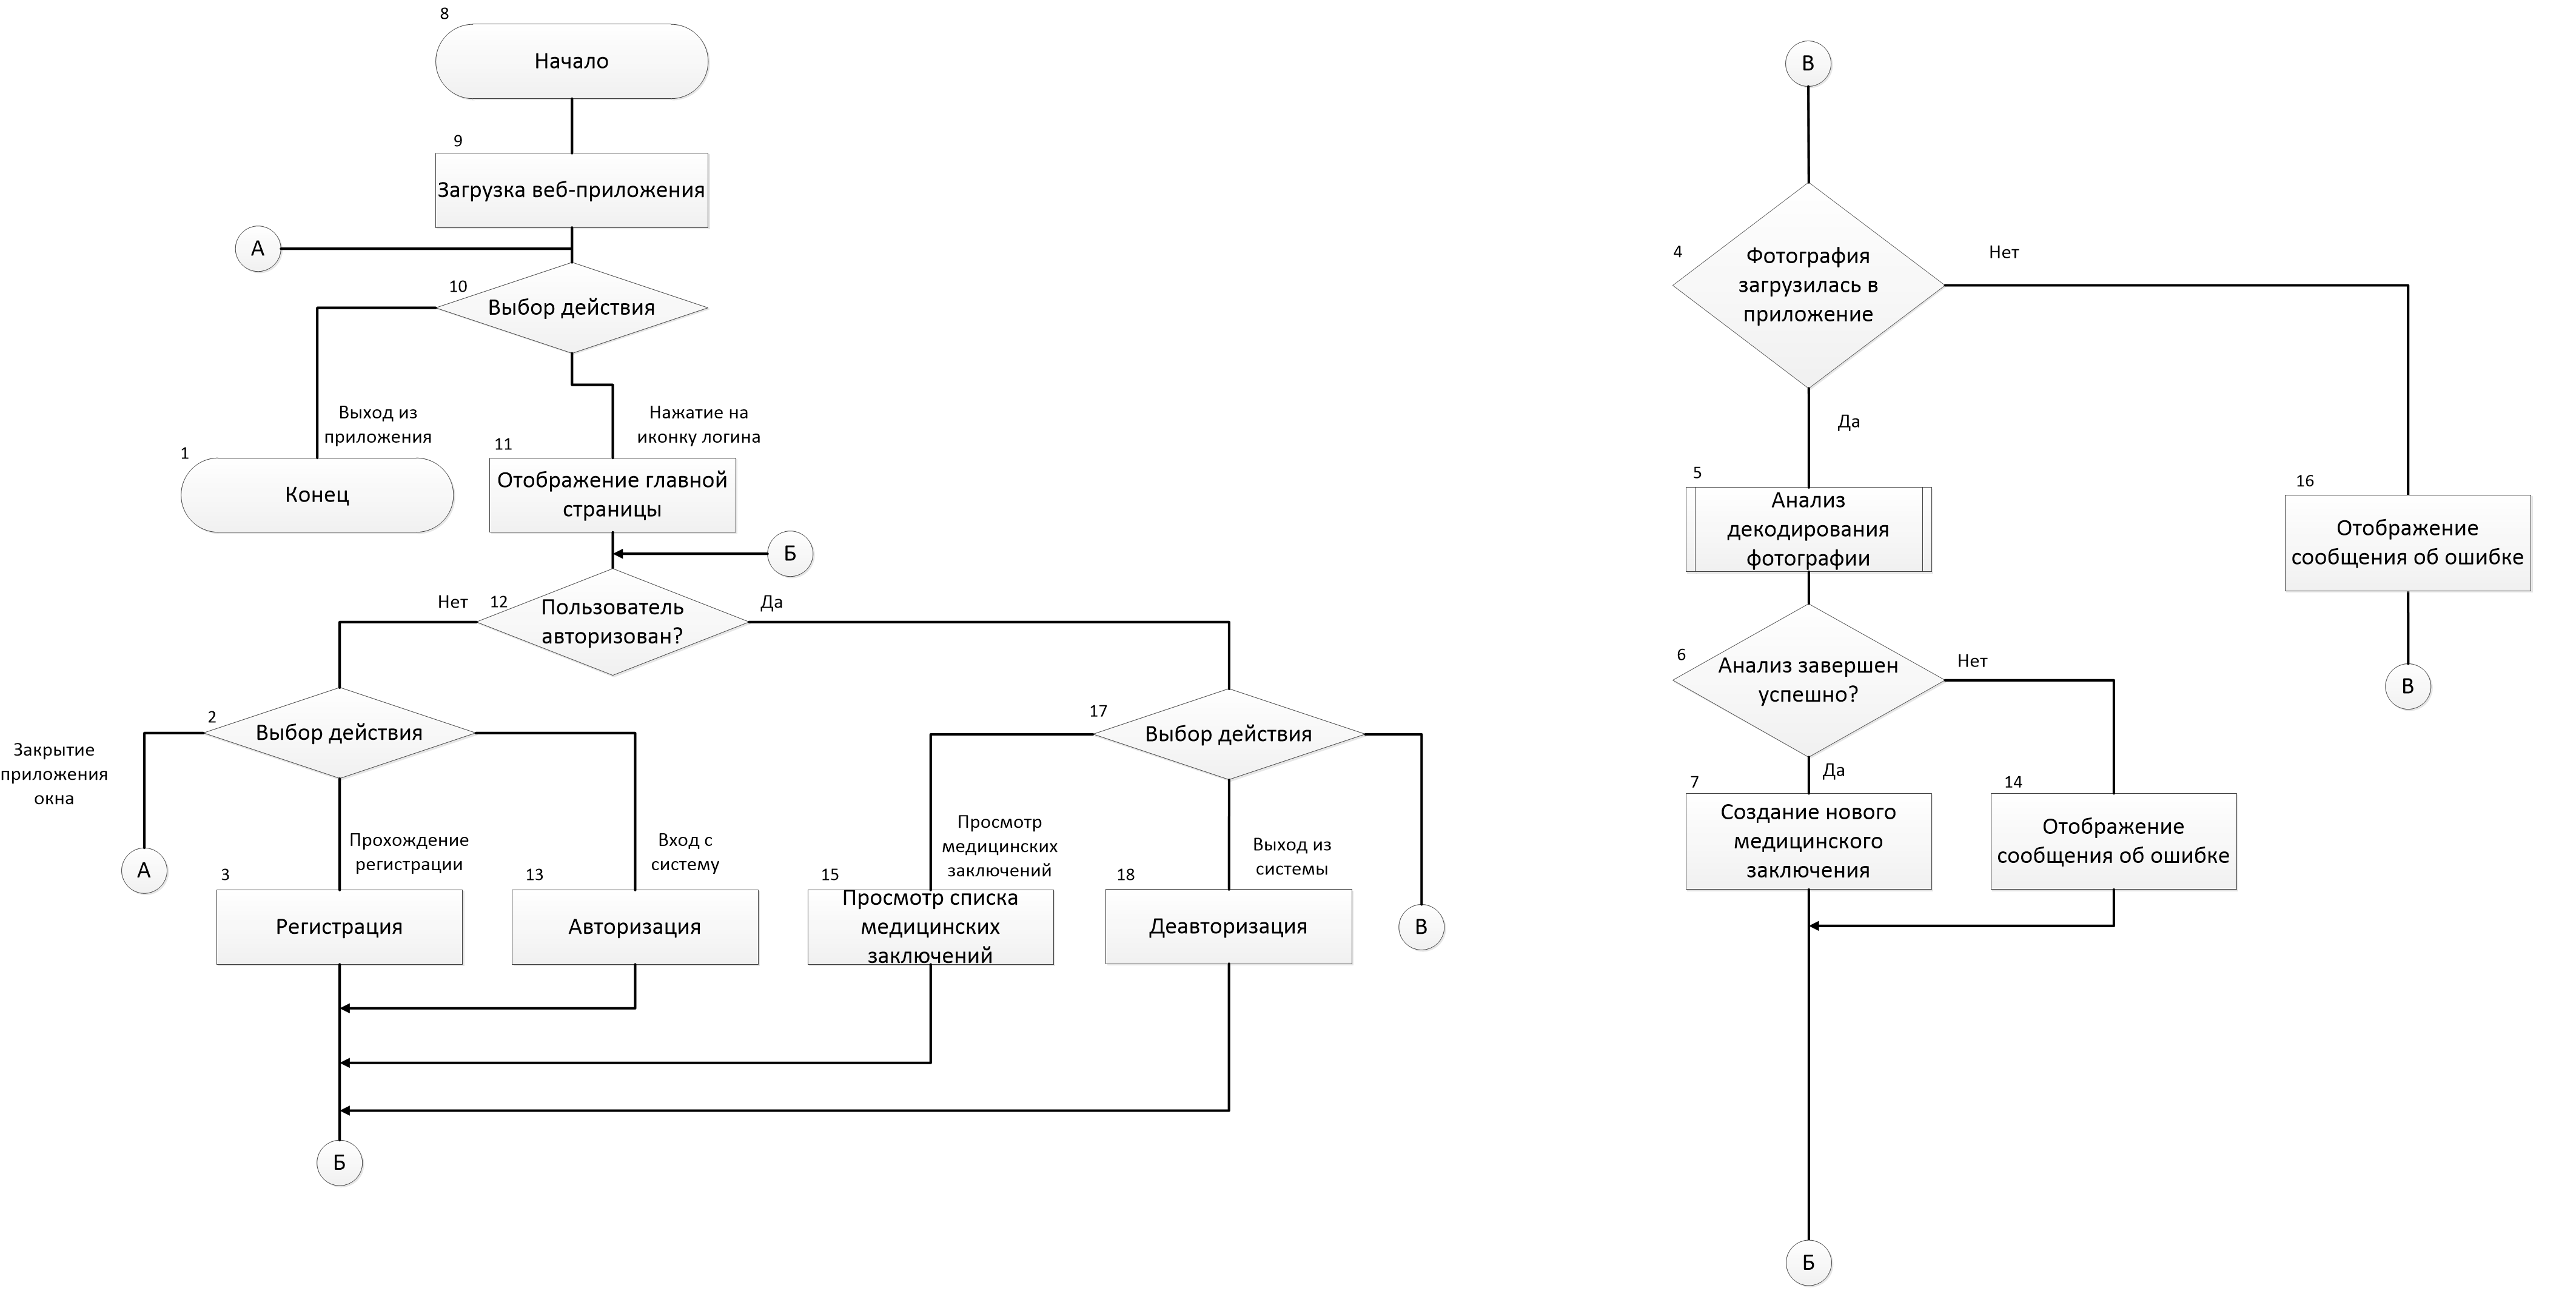
\includegraphics[scale=0.25]{spAlho.png}  
  \caption{ Схема работы программы. }
  \label{fig:domain:manual_structure:alho_sp}
\end{figure}
\subsection{Разработка алгоритма крипто-сервиса }
\label{sub:arch_and_mod:alholib-crypto}

В дипломном проекте необходимо передавать данные от серверной части к клиентской. Чтобы не произошел перехват данных и их изменения необходимо разработать крипто-сервис, который обеспечит сохранность и достоверность информации, передаваемой от сервера к клиенту.

Для этого был разработан алгоритм AES-128 - симметричный алгоритм блочного шифрования. Этот алгоритм преобразует один 128-битный блок в другой, используя секретный ключ который нужен для такого преобразования. Для расшифровки полученного 128-битного блока используют второе преобразование с тем же секретным ключом.

Размер блока всегда равен 128 бит. Размер ключа также имеет фиксированный размер. Чтобы зашифровать произвольный текст любым паролем можно поступить так: 

\begin{itemize}
  \item получить хеш от пароля;
  \item преобразовать хеш в ключ по правилам описанным в стандарте AES;
  \item разбить текст на блоки по 128 бит;
  \item зашифровать каждый блок функцией cipher;
\end{itemize}
\begin{figure}[ht]
\centering
  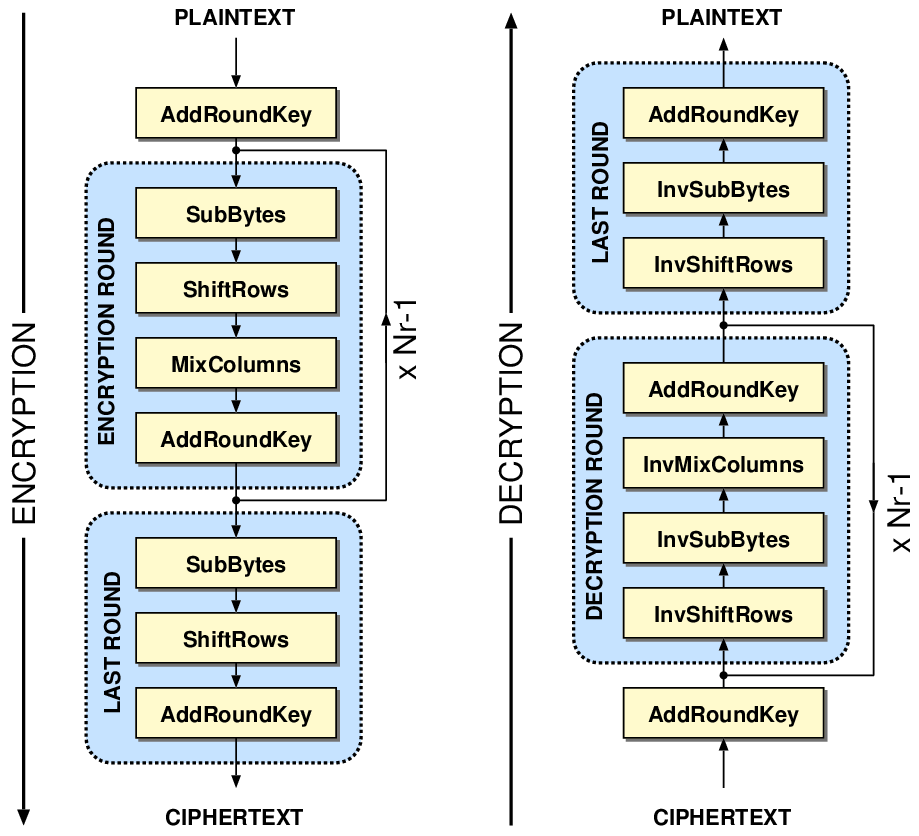
\includegraphics[scale=0.5]{alho_aes.png}  
  \caption{ Структура алгоритма AES. }
  \label{fig:domain:manual_structure:structural_aes}
\end{figure}
На рисунке ~\ref{fig:domain:manual_structure:structural_aes} представлен алгоритм шифрования на вход которого приходит 128-битный блок данных plaintext и расписание ключей w, которое получается после KeyExpansion. 16-байтый plaintext он записывает в виде матрицы s размера 4*Nb, которая называется состоянием AES, и затем Nr раз применяет к этой матрице 4 преобразования. В конце он записывает матрицу в виде массива и подаёт его на выход — это зашифрованный блок. Каждое из четырёх преобразований очень простое.

AddRoundKey берёт из расписания ключей одну матрицу размера 4*Nb и поэлементно добавляет её к матрице состояния. Если два раза применить AddRoundKey, то ничего не изменится, поэтому преобразование обратное к AddRoundKey это оно само.

SubBytes заменяет каждый элемент матрицы состояния соответвующим элементом таблицы SBox: sij = SBox[sij]. Преобразование SubBytes обратимо. Обратное к нему находится с помощью таблицы InvSBox.

ShiftRows сдвигает i-ую строку матрицы s на i позиций влево, считая i с нуля. Обратное преобразование InvShiftRows сдвигает строки вправо.

MixColumns умножает каждый столбец матрицы s слева на особую матрицу размера 4*4:
